% C4AI4C'27 (ICASSP 2027 Satellite Workshop) -- full manuscript, version final_v1.
% Official ICASSP 2027 template (spconf.sty, IEEEbib.bst). Limit: 4 pages of content; page 5 may hold only
% references, the ethics statement and acknowledgments. Every number is taken from the frozen artifacts
% (exports/ICASSP2027_revision_v2, unified_outcomes*.json, claim ledger paper_plan/04).
\documentclass{article}
\usepackage{spconf,amsmath,amssymb,graphicx,booktabs,algorithm,algpseudocode,url}
\usepackage[hidelinks]{hyperref}

\newcommand{\vthree}{FedTrace~v3}
\newcommand{\Wone}{W1$^\ast$}
\newcommand{\Wtwo}{W2$^\ast$}

\title{Detection Is Not Attribution: A Reliability Study of Federated Learning Forensics Under Poisoning and Benign Drift}

\twoauthors
  {Al Amin}
  {Huston--Tillotson University\\
   Austin, TX, USA\\
   \texttt{EMAIL-TO-CONFIRM@htu.edu}}
  {Kamrul Hasan, Liang Hong}
  {Tennessee State University\\
   Nashville, TN, USA\\
   \texttt{\{mhasan1, lhong\}@tnstate.edu}}

\begin{document}
\ninept
\maketitle

\begin{abstract}
An anomalous client update in federated learning (FL) is not proof that the client is malicious. We audit
\vthree, a frozen server-side forensic monitor from our earlier work, alongside three sequential norm detectors.
The setting is a five-client CIFAR-100 setup with matched clean, BadNets, relabel-only and honest class-drift arms,
run over four seeds, two of them preregistered. Attack success, detection, first-source attribution, onset error
and honest-client accusations are reported separately. \vthree{} raises no alarm in any clean run, but it misses
the BadNets attacker in both preregistered runs, including one with 63.3\% attack success. Norm z-score persistence
and CUSUM use the same norm statistic with a lower threshold. They attribute the attacker in all four BadNets runs,
yet accuse honest clients in every drift arm and in one preregistered clean run. In one development seed, an
inclusive-median reference effect explains six honest accusations. We document seed-level failures, not a new
detector or population error rates.
\end{abstract}

\begin{keywords}
Federated learning, forensic attribution, data poisoning, benign drift, change detection
\end{keywords}

% ============================================================================================================
\section{Introduction}
\label{sec:intro}

Federated learning (FL) trains a shared model from client updates without collecting raw data~\cite{mcmahan2017fedavg}.
Because the server sees each client's update, it can monitor clients and react to anomalies by excluding a client
or rolling back a round. Such monitoring is hard for two reasons. First, heterogeneous local data already make
benign updates diverse~\cite{li2020fedprox,karimireddy2020scaffold}. Second, poisoning can implant targeted
backdoors~\cite{gu2019badnets,bagdasaryan2020backdoor} or produce persistent multi-round
deviations~\cite{xie2025multiround}.

A server-side forensic verdict bundles several distinct questions. Was the intervention effective? Was the
responsible client detected? Was the \emph{correct} client named first? When did the intervention begin? Were honest
clients accused? A single detection score hides these distinctions, and in few-client cross-silo FL they carry
real weight: with five participants, one false exclusion removes 20\% of the federation.

We audit \vthree, a server-side monitor that we developed earlier for model-update perturbations
(Fig.~\ref{fig:overview}). Its detector and thresholds are frozen; we do not modify them. Our contributions are:
\begin{itemize}
  \item a matched audit design: four interventions on one client with bit-identical pre-intervention histories,
        five separately reported outcomes, and confirmation seeds preregistered before the run;
  \item seed-level evidence of a detection--specificity trade-off, isolated by comparing one norm statistic at two
        frozen thresholds;
  \item a conditional analysis of peer-reference contamination. An exact median identity explains all six honest
        accusations in one seed, and the identity's precondition is absent in the other three.
\end{itemize}
Separating these outcomes is not new in itself: FLDetector reports client-level errors and FLTracer reports
provenance and timing~\cite{zhang2022fldetector,zhang2024fltracer}. We report every outcome, including
ineffective attacks, missed attackers and false accusations.

% ============================================================================================================
\section{Relation to Prior Work}
\label{sec:prior}

Robust aggregation such as Krum~\cite{blanchard2017krum} limits the influence of outliers but does not name a
responsible client. DeepSight inspects model-update features to filter backdoored
models~\cite{rieger2022deepsight}. CrowdGuard relies on client-side validation~\cite{rieger2024crowdguard}, and
BackdoorIndicator probes server-injected indicator tasks~\cite{li2024backdoorindicator}. FedREDefense uses
model-update reconstruction error and targets crafted model poisoning rather than arbitrary local-data
poisoning~\cite{xie2024fedredefense}. Among methods that name clients, FLDetector predicts each client's update from
its history~\cite{zhang2022fldetector}. FLTracer attributes poisoning online with attack time and type, and notes
that abruptly changing benign clients remain difficult~\cite{zhang2024fltracer}. FLForensics traces clients
retrospectively from a misclassified target input~\cite{jia2025flforensics}. FoolsGold addresses colluding
Sybils~\cite{fung2020foolsgold}, FLTrust uses a trusted server dataset~\cite{cao2021fltrust}, and FedGT identifies
malicious clients under secure aggregation~\cite{xhemrishi2025fedgt}. Our baselines are classical sequential change
detectors~\cite{page1954cusum,hinkley1971changepoint}. We did not run any of the published forensic systems, so we
make no numerical comparison with them.

% ============================================================================================================
\section{Frozen Monitor and Baselines}
\label{sec:monitor}

\begin{figure*}[t]
\centering
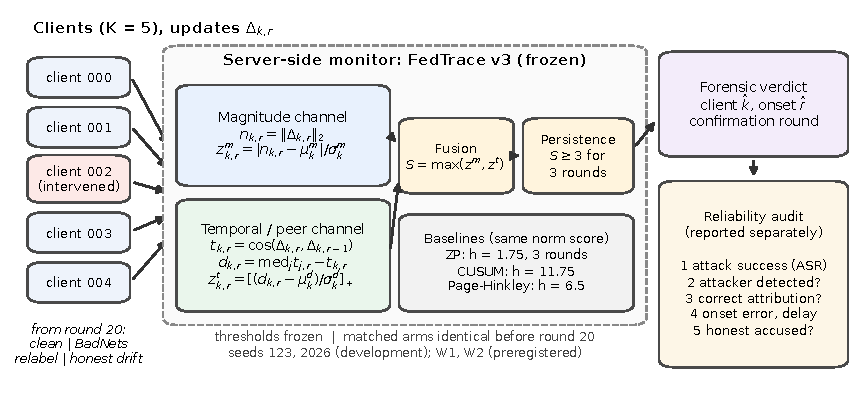
\includegraphics[width=0.94\textwidth]{figures/fig_overview.pdf}
\vspace{-2mm}
\caption{\textbf{Audited pipeline and audit outcomes.} Five clients send identity-labelled updates; client 002 is
intervened on from round 20 (clean, BadNets, relabel-only or honest drift), and all arms are identical before round
20. The frozen \vthree{} monitor combines a magnitude score and a temporal/peer score, fuses them by maximum, and
confirms a client after three consecutive rounds with $S\ge3$. The norm baselines use the same norm score. Each run
is audited for attack success, detection, first attribution, onset error and delay, and honest accusations.}
\label{fig:overview}
\vspace{-3mm}
\end{figure*}

At round $r$ the server observes each client's identity-labelled update $\Delta_{k,r}\in\mathbb{R}^d$ but not its
data. Let $n_{k,r}=\|\Delta_{k,r}\|_2$ be the update norm and
$t_{k,r}=\langle\Delta_{k,r},\Delta_{k,r-1}\rangle/(\|\Delta_{k,r}\|_2\|\Delta_{k,r-1}\|_2)$ the self-cosine. With
the inclusive peer median $c_r=\mathrm{med}_j\,t_{j,r}$ and the residual $d_{k,r}=c_r-t_{k,r}$, the frozen score is
\begin{equation}
z^m_{k,r}=\frac{|n_{k,r}-\mu^m_k|}{\sigma^m_k},\quad
z^t_{k,r}=\max\Big(0,\frac{d_{k,r}-\mu^d_k}{\sigma^d_k}\Big),\quad
S_{k,r}=\max\{z^m_{k,r},z^t_{k,r}\}.
\label{eq:score}
\end{equation}
Per-client sample means and standard deviations are calibrated on rounds $0$--$19$ for the norm and $1$--$19$ for
the residual ($T_{\mathrm{ref}}=20$). The magnitude score is two-sided, so unusually small and unusually large
updates both count. Algorithm~\ref{alg:fedtrace} gives the confirmation, attribution and onset rules ($\tau=3$,
$P=3$).

\begin{algorithm}[t]
\small
\caption{\vthree{} forensic monitor (frozen; evaluated, not proposed)}
\label{alg:fedtrace}
\begin{algorithmic}[1]
\Require updates $\Delta_{k,r}$, $k=1,\dots,K$; $T_{\mathrm{ref}}=20$; $\tau=3$; $P=3$
\Statex \textbf{Calibration} (once, at $r=T_{\mathrm{ref}}$)
\For{each client $k$}
  \State $\mu^m_k,\sigma^m_k\gets$ mean, s.d.\ of $n_{k,r}$, $0\le r<T_{\mathrm{ref}}$
  \State $\mu^d_k,\sigma^d_k\gets$ mean, s.d.\ of $d_{k,r}$, $1\le r<T_{\mathrm{ref}}$
\EndFor
\Statex \textbf{Monitoring} (each round $r\ge T_{\mathrm{ref}}$)
\For{each client $k$}
  \State compute $z^m_{k,r}$, $z^t_{k,r}$ and $S_{k,r}$ by Eq.~(\ref{eq:score})
  \If{$S_{k,r'}\ge\tau$ for $r'=r-P+1,\dots,r$ \textbf{and} $k$ unconfirmed}
    \State confirm $k$ at round $r$; onset estimate $\hat r_k\gets r-P+1$
  \EndIf
\EndFor
\State \Return first-attributed client $\hat k$: earliest confirmation (ties: larger mean streak score); $\hat r_{\hat k}$; all confirmations
\end{algorithmic}
\end{algorithm}

\textbf{Baselines.} All three baselines run on the per-client norm. Norm z-score persistence (ZP) confirms a
client after $P=3$ consecutive rounds above $h=1.75$. CUSUM uses $h=11.75$ and $\kappa=0.5$~\cite{page1954cusum},
and Page--Hinkley (PH) uses $h=6.5$ and $\delta=0.5$~\cite{hinkley1971changepoint}. Each threshold is the smallest
grid value with no alarm on the two development clean runs, which is the most sensitive operating point consistent
with those runs; it is not a false-alarm guarantee. The ZP statistic is numerically identical to $z^m$ (maximum
difference 0 on all evaluated traces). ZP and the magnitude channel of \vthree{} therefore differ only in threshold
(1.75 vs.\ 3). We also run five ablations of \vthree: magnitude-only; temporal-only; and leave-one-out,
trimmed-mean and client-historical reference variants.

% ============================================================================================================
\section{Matched Interventions and Outcomes}
\label{sec:protocol}

\textbf{Setting.} 50-round FedAvg on CIFAR-100~\cite{krizhevsky2009cifar} with a CIFAR-style
ResNet-18~\cite{he2016resnet}, $K=5$ fully participating clients, Dirichlet $\alpha=0.1$ partitions, one local
epoch, SGD (learning rate 0.01, batch 32), and a 45k/5k train/validation split. Client 002 is intervened on from
round $r^\star=20$. Within a seed, all arms share bit-identical pre-intervention histories (21 global states and 100
client submissions). Seeds 123 and 2026 were used for development. Confirmation seeds W1 (1178015705) and W2
(1463065807) were drawn by a fixed SHA-256 rule and preregistered with all thresholds frozen; we mark them
\Wone{} and \Wtwo. Under \Wone, client 002 holds 347 target-class samples, a disclosed difference from the
development seeds.

\textbf{Interventions.} \emph{BadNets}~\cite{gu2019badnets} adds a $3\times3$ trigger and relabels 50\% of client
002's non-target-class samples to target class 0. Attack success rate (ASR) is measured on 9,900 triggered
non-target test images, with a preregistered effectiveness criterion of ASR $\ge 50\%$. \emph{Relabel-only} uses
the same samples and label without the trigger (development seeds only). \emph{Honest drift} keeps a set of client
002's classes covering at least 50\% of its samples and replaces each sample of the other classes with a correctly
labelled sample of a retained class from the same client. Dataset length and optimizer steps are unchanged. This
is a constructed stress test, not an estimate of how common benign drift is.

\textbf{Outcomes.} For attacked runs we record, separately, whether the attacker is ever confirmed (detection);
whether it is the first confirmed client (attribution); the onset error $e=|\hat r-r^\star|$; the delay
$d=r_{\mathrm{confirm}}-r^\star$; and whether any honest client is also confirmed (FA). In clean and drift arms
every confirmation is a false accusation. Missed attackers receive no onset error.

% ============================================================================================================
\section{Results}
\label{sec:results}

\begin{table*}[t]
\centering\footnotesize
\setlength{\tabcolsep}{5pt}
\renewcommand{\arraystretch}{1.02}
\caption{\textbf{Seed-level outcomes} (no pooling). \checkmark$(e,d)$: attacker confirmed first, with onset error
$e$ and delay $d$ in rounds (a checkmark does not exclude later honest confirmations). W: honest client(s) confirmed
first. M: attacker never confirmed. FA$\{i\}$: honest client(s) $i$ confirmed. --: no client confirmed.
n/r: not run. $^\ast$preregistered confirmation seed. Accuracy changes are relative to the matched clean run.}
\label{tab:main}
\vspace{-1mm}
\begin{tabular}{@{}llcccc@{}}
\toprule
Arm & Quantity / detector & 123 & 2026 & \Wone & \Wtwo \\
\midrule
Clean & top-1 accuracy (\%) & 56.88 & 57.94 & 58.04 & 60.22 \\
 & \vthree & -- & -- & -- & -- \\
 & ZP, CUSUM, PH (each) & -- & -- & FA\{4\} & -- \\
\midrule
BadNets & ASR (\%) / top-1 change (pp) & 43.5 / $-1.94$ & 64.7 / $-0.94$ & 63.3 / $-0.96$ & 44.2 / $-0.86$ \\
 & \vthree & \checkmark$(8,10)$ & W: FA\{1,4\} first; attacker later ($d{=}4$) & M & M \\
 & ZP & \checkmark$(1,3)$ & \checkmark$(0,2)$ & \checkmark$(1,3)$+FA\{4\} & \checkmark$(1,3)$ \\
 & CUSUM & \checkmark$(0,6)$ & \checkmark$(0,5)$ & \checkmark$(0,6)$+FA\{4\} & \checkmark$(0,6)$ \\
 & Page--Hinkley & M+FA\{0\} & M+FA\{1\} & M+FA\{4\} & M \\
\midrule
Relabel-only & ASR (\%) / top-1 change (pp) & 0.7 / $-1.26$ & 0.4 / $-1.60$ & n/r & n/r \\
 & \vthree & M & M+FA\{1,4\} & n/r & n/r \\
 & ZP & \checkmark$(1,3)$ & \checkmark$(1,3)$ & n/r & n/r \\
 & CUSUM & \checkmark$(0,7)$ & \checkmark$(0,6)$ & n/r & n/r \\
 & Page--Hinkley & M & M+FA\{1\} & n/r & n/r \\
\midrule
Honest drift & top-1 change (pp) & $-1.75$ & $-1.79$ & $-2.29$ & $-1.47$ \\
 & \vthree & -- & FA\{1,4\} & FA\{2\} & -- \\
 & ZP & FA\{2\} & FA\{1\} & FA\{2,4\} & FA\{2\} \\
 & CUSUM & FA\{2\} & FA\{2\} & FA\{2,4\} & FA\{2\} \\
 & Page--Hinkley & -- & FA\{1\} & FA\{4\} & -- \\
\bottomrule
\end{tabular}
\vspace{-3mm}
\end{table*}

\textbf{Effective attacks can be missed.} Table~\ref{tab:main} lists every outcome. BadNets exceeds the 50\%
criterion only in seeds 2026 and \Wone; we keep the two weaker runs (43.5\% and 44.2\%) rather than drop them.
\vthree{} attributes the attacker late at seed 123 (onset error 8, delay 10). At 2026 it confirms honest clients
001 and 004 at round 23, one round before the attacker. It never confirms the attacker in \Wone{} or \Wtwo, even
though \Wone{} reaches 63.3\% ASR. The relabel-only arms show the converse dissociation: ASR stays at 0.7\% and
0.4\%, yet ZP and CUSUM confirm the intervened client. An alarm therefore does not show that a backdoor succeeded,
and a successful backdoor need not raise an alarm.

\textbf{One statistic, two thresholds.} Fig.~\ref{fig:calibration}(a) shows why the norm baselines and \vthree{}
diverge. The attacker's norm score peaks at 3.26, 3.57, 3.04 and 2.94 (seeds 123, 2026, \Wone, \Wtwo). It is at
least 3 in 10, 21, 2 and 0 rounds, but above 1.75 in 29, 30, 29 and 29 of the 30 post-onset rounds. On the
confirmation seeds it therefore never sustains three consecutive rounds at $\tau=3$, while ZP, using the identical
statistic, confirms the attacker on every seed. Including the first two high-norm training rounds in calibration
inflates $\sigma^m$ by 1.8--7.1$\times$ across clients on the development seeds. For the attacker the inflation is
6.3--7.1$\times$ in three seeds and 1.9$\times$ in \Wone. This is consistent with the misses, but we did not test it
as a cause. Since \vthree{} also fuses the temporal channel, its full decisions are not explained by the threshold
alone.

\begin{figure}[t]
\centering
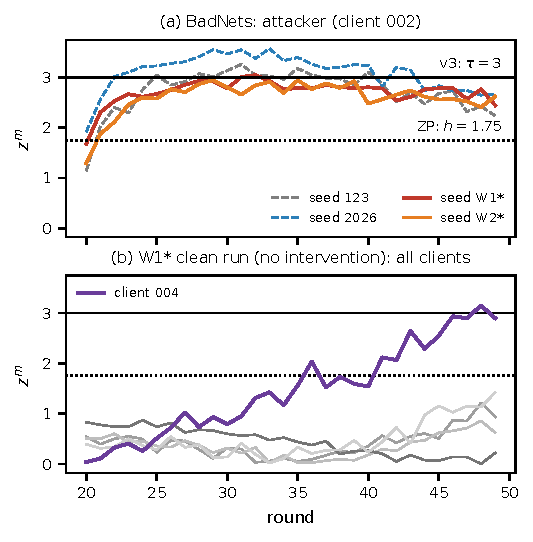
\includegraphics[width=\columnwidth]{figures/fig_calibration_col.pdf}
\vspace{-6mm}
\caption{\textbf{Norm score $z^m$ after onset.} (a) BadNets attacker, four seeds. On \Wone{} and \Wtwo{} the score
stays between the ZP threshold ($h=1.75$, dotted) and the \vthree{} threshold ($\tau=3$, solid). (b) \Wone{} clean
run: honest client 004 drifts above $h=1.75$ late in training, producing the ZP, CUSUM and PH clean alarm; \vthree{}
raises none.}
\label{fig:calibration}
\vspace{-3mm}
\end{figure}

\textbf{Sensitivity costs specificity.} \vthree{} is silent in all four clean runs. ZP, CUSUM and PH all accuse
client 004 in the \Wone{} clean run, where its norm drifts upward late in training (Fig.~\ref{fig:calibration}(b)).
ZP and CUSUM also accuse an honest client in every drift arm, and \vthree{} does so in 2026 and \Wone. Thresholds
transferred from two development clean runs did not preserve specificity: the ZP threshold lies only 0.031 above the
largest development clean statistic. The calibration data are also strongly dependent. Clean norm scores have
lag-one autocorrelation 0.82--0.91 and mean cross-client correlation 0.94--0.95, giving an AR(1) effective sample
size of only 1.5--2.9 of 30 clean rounds per client.

\begin{table}[t]
\centering\footnotesize
\setlength{\tabcolsep}{2.4pt}
\caption{\textbf{Frozen ablations of \vthree} (same thresholds). BadNets columns: C correct first attribution, W
honest client first, M missed, +FA honest client also confirmed. Last two columns: seeds with an honest
confirmation in the drift and clean arms.}
\label{tab:ablation}
\vspace{-1mm}
\begin{tabular}{@{}lccccll@{}}
\toprule
Variant & 123 & 2026 & \Wone & \Wtwo & Drift FA & Clean FA \\
\midrule
Full \vthree & C & W & M & M & 2026, W1 & none \\
Magnitude only & C & C & M & M & W1 & none \\
Temporal only & M & M+FA & M & M & 2026 & none \\
Leave-one-out ref. & W & C & M+FA & M & 123, W1 & none \\
Trimmed-mean ref. & W & C & M+FA & M & 123, W1 & none \\
Historical ref. & C+FA & C+FA & M+FA & M+FA & all & all \\
\bottomrule
\end{tabular}
\vspace{-3mm}
\end{table}

\textbf{No ablation is uniformly safe.} Table~\ref{tab:ablation} varies one component at a time. Magnitude-only
fixes the 2026 first-attribution error but still misses both confirmation attackers. Temporal-only misses every
BadNets attacker and accuses the same honest clients at 2026. Leave-one-out and trimmed-mean references also fix
2026, but they move the error to seed 123, where honest client 001 is confirmed first. The client-historical
reference accuses honest clients in every clean run. Choosing whichever variant looks best afterwards would
therefore overstate reliability.

% ============================================================================================================
\section{Conditional Reference Contamination}
\label{sec:contamination}

\begin{figure*}[t]
\centering
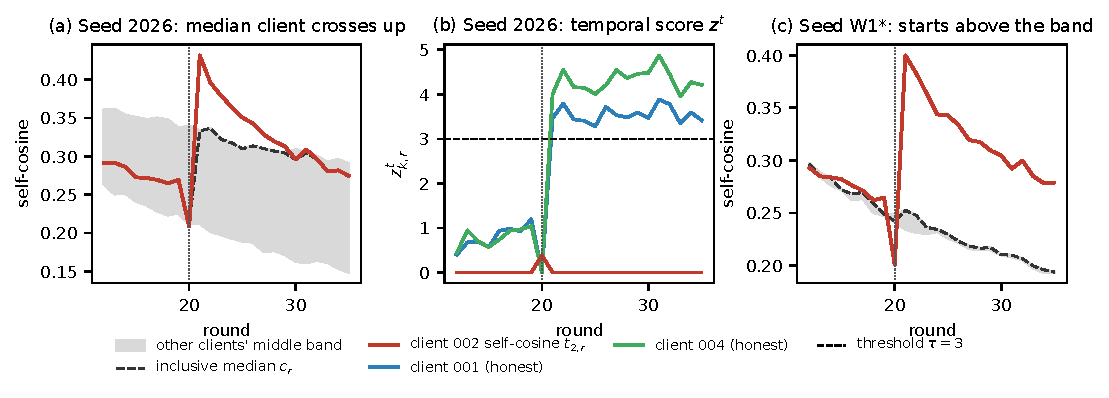
\includegraphics[width=0.92\textwidth]{figures/fig_contamination.pdf}
\vspace{-2mm}
\caption{\textbf{Reference contamination requires a rank crossing.} (a) Development seed 2026, BadNets: client 002
starts as the median client; after onset its self-cosine rises through the other clients' middle band and drags the
inclusive median $c_r$ upward. (b) Honest clients 001 and 004 receive temporal scores above $\tau=3$ and are
confirmed at round 23, while client 002's own temporal score stays at 0. (c) Preregistered seed \Wone: client 002
starts above the band, so its rise leaves the median unchanged.}
\label{fig:contamination}
\vspace{-3mm}
\end{figure*}

Why does \vthree{} accuse honest clients first at 2026? Let $j$ be the intervened client with $x=t_{j,r}$, and hold
the other clients' self-cosines fixed, sorted as $s_1\le\dots\le s_{K-1}$. For odd $K=2m-1$ the inclusive median is
\begin{equation}
c(x)=\min\{\max\{x,s_{m-1}\},s_m\},\qquad \Delta d_{k,r}=\Delta c_r\ \ (k\neq j).
\label{eq:clip}
\end{equation}
By Eq.~(\ref{eq:clip}), client $j$ moves the reference only by crossing the band $[s_{m-1},s_m]$, and every honest residual then shifts by
the same $\Delta c_r$. Because $z^t$ is one-sided, this shift raises an honest score only while that score is
positive, and a false accusation still needs a full confirming streak. The identity itself is elementary; what
matters forensically is when its precondition holds. At 2026, client 002 was the median client before onset (rank
3 of 5). Its self-cosine jumped to 0.43 at round 21, moving $c_r$ from 0.257 in the matched clean run to 0.333
(Fig.~\ref{fig:contamination}). The standardized residuals of honest clients rose by $+1.3$ to $+2.4$ (mean over
rounds 20--29), almost entirely through the reference. Clients 001 and 004 reached temporal scores of 3.5 and 4.0 at
round 21 and were confirmed at round 23. Removing client 002's displacement retrospectively breaks at least one
round of each of the six affected honest streaks (three arms $\times$ two clients). A source-agnostic baseline, the
reference's movement relative to its calibration mean, breaks three of the six. In seeds 123, \Wone{} and \Wtwo{}
client 002 started at rank 4, so the upward-crossing precondition never arose. A deployable proxy for the
displacement had mean error 0.07$z$ in development but 0.6--2.7$z$ in confirmation, so it is not a usable
correction. This is a conditional, one-seed explanation, not evidence that the same effect caused the \Wone{} and
\Wtwo{} misses.

% ============================================================================================================
\section{Archived Model-Update Perturbations}
\label{sec:archived}

\begin{table}[t]
\centering\footnotesize
\setlength{\tabcolsep}{3pt}
\caption{\textbf{Archived model-update perturbations} (not data poisoning), frozen \vthree. Onset error / delay in
rounds; all first attributions correct.}
\label{tab:archived}
\vspace{-1mm}
\begin{tabular}{@{}llc@{}}
\toprule
Setting (FedAvg) & Seeds & $e$ / $d$ \\
\midrule
Gaussian noise $\rho=1$, $K=5$ & 123, 2026 & 0/2, 0/2 \\
Norm-preserving directional $c=0$, $K=5$ & 123, 2026 & 0/2, 0/2 \\
Directional, attacker 004 / onset at round 30 & 123 & 0/2, 0/2 \\
Gaussian / directional, $K=10$ & 123 & 0/2, 0/2 \\
Reduced severity: Gaussian $\rho=0.5$ & 123 & 21/23 \\
Reduced severity: directional $c=0.5$ & 123 & 0/2 \\
Intermittent Gaussian / directional & 123 & 0/2, 0/2 \\
\midrule
Ablation: magnitude only, directional & 123, 2026 & 27/29, 24/26 \\
Ablation: temporal only, Gaussian & 123, 2026 & 1/3, 0/2 \\
\bottomrule
\end{tabular}
\vspace{-3mm}
\end{table}

For context, Table~\ref{tab:archived} recomputes the same frozen monitor on our archived traces, where an attacker
perturbs its model update directly after local training. That threat model is different, and these runs are not
additional BadNets replications. Under it, \vthree{} attributes the attacker with onset error 0 and delay 2 in
every setting except reduced-severity Gaussian noise. Each channel covers a perturbation the other handles poorly.
In an archived four-run sweep, persistence $P=2$ produced honest alarms at $\tau\in\{2.5,3\}$, while $P\ge3$
produced none for $\tau\in\{2.5,3,3.5\}$. Under Multi-Krum aggregation, however, \vthree{} confirms an honest client
in both archived clean runs (first at round 46), driven by a slow upward norm drift. Those runs executed code that
is not contained in their recorded commit, which is a provenance caveat. Success on synthetic update perturbations
did not carry over to local-data poisoning.

% ============================================================================================================
\section{Discussion, Limitations and Conclusion}
\label{sec:conclusion}

\textbf{Why intent is hard to read from updates.} For any binary decision $\phi$ between malicious and admissible
benign observation laws $P_M$ and $P_B$, $P_B(\phi=1)+P_M(\phi=0)\ge 1-\mathrm{TV}(P_B,P_M)$. When the laws are
close, no decision rule can make both errors small without further assumptions about benign behaviour. Our
constructed drift shows a practical version of this ambiguity: a correctly labelled change in class composition
produced the same norm signature that the baselines use to catch BadNets. It does not show that the two laws are
equal. In practice, a confirmed anomaly should be treated as a lead rather than proof. A forensic report should keep
the full alarm timeline, separate first attribution from later confirmations, and include clean and benign-change
controls whenever a threshold is set.

\textbf{Limitations.} The evidence comes from four matched seeds in one setting (CIFAR-100, ResNet-18, $K=5$,
Dirichlet $\alpha=0.1$) with one intervened client and one constructed drift, so it does not support population
error rates. Two BadNets runs fall below the 50\% criterion. The onset $r^\star=20$ coincides with the end of the
calibration window, so other onset times remain untested. The contamination explanation rests on one development
seed. We did not execute published forensic systems as comparators. The monitor needs identity-labelled individual
updates, which secure aggregation hides.

\textbf{Conclusion.} The matched controls separate backdoor effectiveness, eventual detection, first-source
attribution, onset estimation and honest accusations, and these outcomes disagreed repeatedly. A stricter frozen
threshold avoided clean alarms but missed effective attacks. A more sensitive threshold on the same statistic caught
every attacker but accused honest drifting clients. Reliability claims for FL forensics should therefore report
each outcome, seed by seed, together with benign controls.

% ---- page 5: only the ethics statement, acknowledgments and references ----
\section{Compliance with Ethical Standards}
This is a numerical simulation study on the public CIFAR-100 dataset. No human subjects or personal data were
involved, and no ethical approval was required.

\section{Acknowledgments}
% PI: add funding sources, or state that there was no external funding.
In accordance with the IEEE policy on AI-generated content, we disclose the following. Claude (Anthropic) wrote the
analysis and evaluation code for the matched interventions, baselines, ablations and contamination analysis. Under
author supervision it also executed the development and confirmation runs, generated all figures, tables and
Algorithm~\ref{alg:fedtrace} from the frozen artifacts, and drafted and edited the manuscript text. ChatGPT (OpenAI)
assisted with earlier drafts of the text. The authors designed the study, approved all protocols before outcomes
were observed, verified every reported number against the experiment artifacts, and take full responsibility for
the content.
% PI: state the AI involvement, if any, in the original FedTrace v1--v3 development.

\bibliographystyle{IEEEbib}
\bibliography{refs}

\end{document}
